\section{Model-View-Controller}

Model-view-controller is a design pattern used by developers. The 
model-view-controller is most commonly used when working on web-applications\cite{mvcasp}. 
The idea of using the model-view-controller is to separate the UI from the 
part of the program that stores the data\cite{modelviewcontroller}. 

The reason why this is a very efficient approach, is that a UI changes a lot more often, 
than the business logic. The MVC-pattern makes it easier to change 
models, views and controllers individually\cite{modelviewcontroller}.

The model-view-controller image looks as follows:

\begin{figure}[ht!]
	\centering
		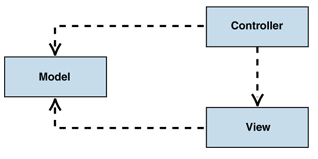
\includegraphics{design/figures/model-view-controller.png}
	\label{fig:model-view-controller}
	\caption{MVC illustration\cite{modelviewcontroller}}
\end{figure}

\subsection{Model-View-Controller Explained}

\noindent
\textbf{Model}

\noindent
The model manages the behavior and data of the application domain. Furthermore, the model objects responds to requests for information about its state (from the view usually). The model also responds to instructions to change state (usually from the controller)\cite{modelviewcontroller}.

\vspace{5 mm}
\noindent
\textbf{View}

\noindent
Views are the aspect of the program that is visible to the user (the UI)\cite{mvcasp}. The user interface is created from the model data\cite{mvcasp}. An edit-view would be dependent on the model to supply it with database entries (or as the user would view it, white-textboxes), in which data could be added. 

\vspace{5 mm}
\noindent
\textbf{Controller}

\noindent
The controller interprets the user's keyboard and mouse input and informs the model or view to change accordingly\cite{mvcasp}.
\subsection{Advantages}

The advantages of the lose coupling in the MVC design pattern is that it makes it possible for 
multiple developers to work on different aspects of the application simultaneously. 
Furthermore, since the model is dependant on neither the view nor the controller, the model 
can be created and tested separately\cite{modelviewcontroller}.

Since the model is independant from the views it follows that a user interface can display data from multiple 
views simultaneously. Another advantage is that on a webpage where the user is able to change, for example, the 
color scheme, the shared model remains the same, but the way it is displayed does not - though the data is 
essentially the same\cite{modelviewcontroller}.